\chapter{Implementation}
This implementation phase shows the process of my work. Showing how the project was implemented and the problems that were encountered during its creation along with realisations that caused me to adapt my final product from the initial design. The main resource used throught this project was several guides on the ESP32 by a website that offers guides and projects called 'Random Nerd Tutorials' \cite{RNTMain}

\section {Start of the Implementation Phase (Sprint One)}
When starting the project, the code produced had some initial iterations that were not up to the level expected. One of the biggest problems encountered was around information storage and how to do this effectively and in the correct manner. One such example of this was the standard LED profile array. The main help used in this sprint was a random nerd tutorial on using PWM pins on a ESP32 \cite{ESP32PWM}.

\subsection {LED profile array size}
When the program was still in the first weeks of development, there were problems with the standard LEDs displaying a dim brightness even though the brightness value that had been assigned to the LED was quite high. The problem persisted even after the hardware (the LEDs, resistors and wires) had been replaced. My supervisor suggested using printout statements to identify what value the brightness array was giving to the main lighting loop which revealed the values coming back were a lot lower than the values that had been set. The problem was the array was never initialised which meant values were not being stored in the correct place in the memory which caused random values to be generated instead of the expected stored values. As a solution, a function was created within the object. This function declares the size of the array that is being used before any values are inputted. However, this is limiting due to the fact that once a profile is created, the size of the profile array cannot be edited. A new LED profile has to be created to have a longer profile array.

\subsection {LED and LED profile objects}
As stated in the design and analysis chapters of the report, all the information was stored on objects that were named LED profiles e.g. the display array, duration, trigger and name of the profile. Initially, the plan was to have an object for the LEDs and an object for the LED profile. The LED profile would store everything about what was being displayed and how e.g. the display array, duration, trigger and name of the profile. On the other hand, the LED object stored the LED channel, the pin the LED its attached to and the LED profile object. However, it was decided that the information for the profiles was better stored on the LED profile. This was because when it came to the main lighting loop of the controller, it quickly became confusing when trying to access the information needed to display the correct brightness/colours. This was due to the fact that in order to access the brightness array, the array inside of an object which was inside of another object had to be referenced. This created long lines of code that quickly became very confusing and hard to read.

\begin{figure}[h]
\centering
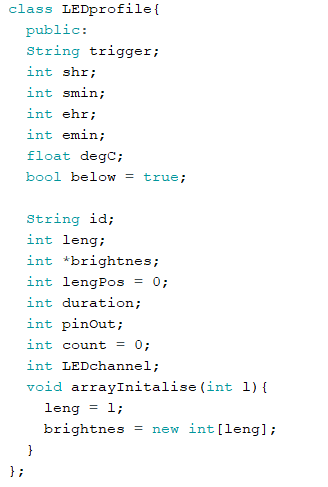
\includegraphics{BLEDProfile}
\end{figure}


\section {Implementing the Addressable LEDs (Sprint Two)}
After these two problems were resolved, the next implementation stage of the project was the use of addressable LEDs. This stage of the project needed to be revised considerably when comparing it to the initial design ideas. The addressable LEDs were not a single LED like the standard LEDs, but a group of LEDs connected in a ring. The solution was to accommodate this by having another object that had an array containing all of the LED profiles for that ring light. In this instance, the ring light that was being tested, had eight LEDs on the ring. So the ring light object had eight assignable LED profiles stored within the LED profile array.

\subsection{Function for the assignable LEDs}
The assignable LEDs used a function called 'Adafruit Neopixel' to display the colours to the ring light. This function required an object to be made and ‘called to’. The function was then able to display colours on the assignable LEDs. Initially, when first implementing the assignable LEDs, it was thought that this object could be created and then ‘called to’ within the ring light object. However, when implemented in this way, the assignable LED always displayed two blue LEDs and one white LED.  This did not alter even if by changing the input variables.  Following extensive research (or trials) it was found that there were no simple/acceptable solutions to this problem.  There was no good acceptable solution to this problem. In order for the assignable LED to work, the object was created outside of the object. As a result the program was restricted to having a specified amount of ring lights prior to the final release to the user. The guide that helped me understand the use of the addressable LEDs was a guide on arduino learning that showed how the libary functioned \cite{WS2812}.

\begin{figure}[h]
\centering
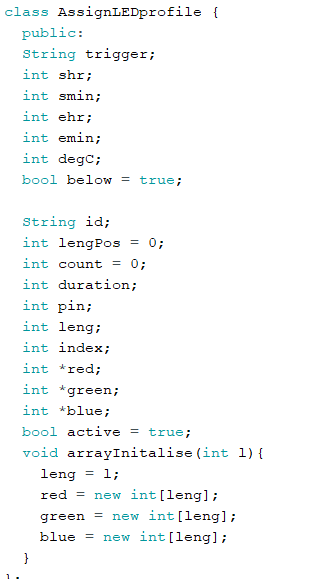
\includegraphics{ColourLEDProfile}
\end{figure}

\newpage

\section{Implementing Triggers (Sprint Three)}
The next implementation stage in the project were the triggers.  The triggers allowed the activation of the LED profiles. Even though this stage was less problematic than other sections of the project, there were some realisations when it came to how the trigger could be activated with the button and the weather sensor.

\subsection {Removing the button trigger}
During this stage it was concluded that the button trigger was not required. One of the negative features of the ESP32 was that there are limitations on the number of pins that can be connected to it. The use of a pin to detect when there was a signal coming from the ESP32 for a trigger seemed very complicated when there was an easier alternative that did not take up an extra pin. When wiring up the LED to the ESP32, a button was added, and the trigger set to constant. The outcome of this was that when the button was pressed the LED is played the profile. However, when the button was pressed, the LED profile did not start at the beginning. It started wherever it was at in the brightness/colour array as the main lighting loop was displaying the colour/brightness to the LEDs even when the button was set to off.

\begin{figure}[h]
\begin{subfigure}{0.5\textwidth}
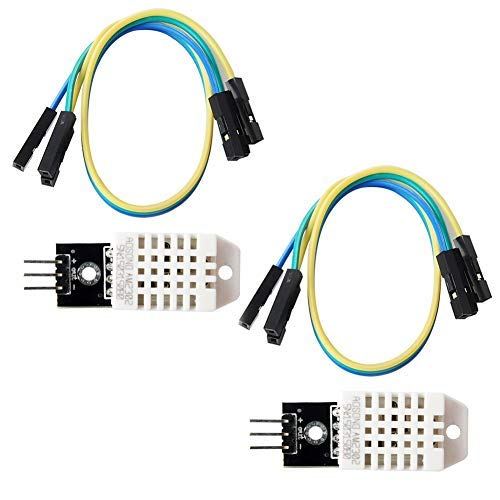
\includegraphics[width=0.9\linewidth, height=6cm]{TempSensor}
\caption{The tempurature sensor used}
\end{subfigure}
\begin{subfigure}{0.5\textwidth}
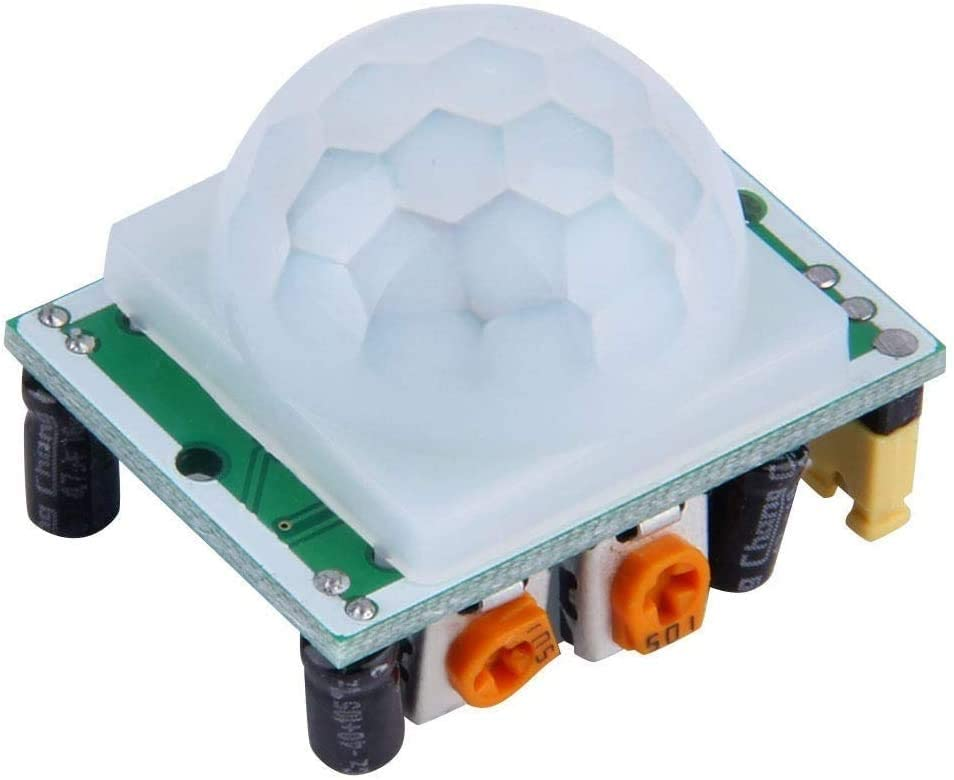
\includegraphics[width=0.9\linewidth, height=7cm]{SensorSensor}
\caption{The sensor used for trigger}
\end{subfigure}
\caption{The two peices of hardware used for the customisable tempurature trigger and the sensor trigger}
\end{figure}

\subsection {Getting and implementing the circuit  boards}
During this week, the circuit boards that were supplied by my supervisor arrived. This did not take too long to implement and reduced the number of wires connected to the board. This made working on the board a lot easier.

\begin{figure}[h]
\centering
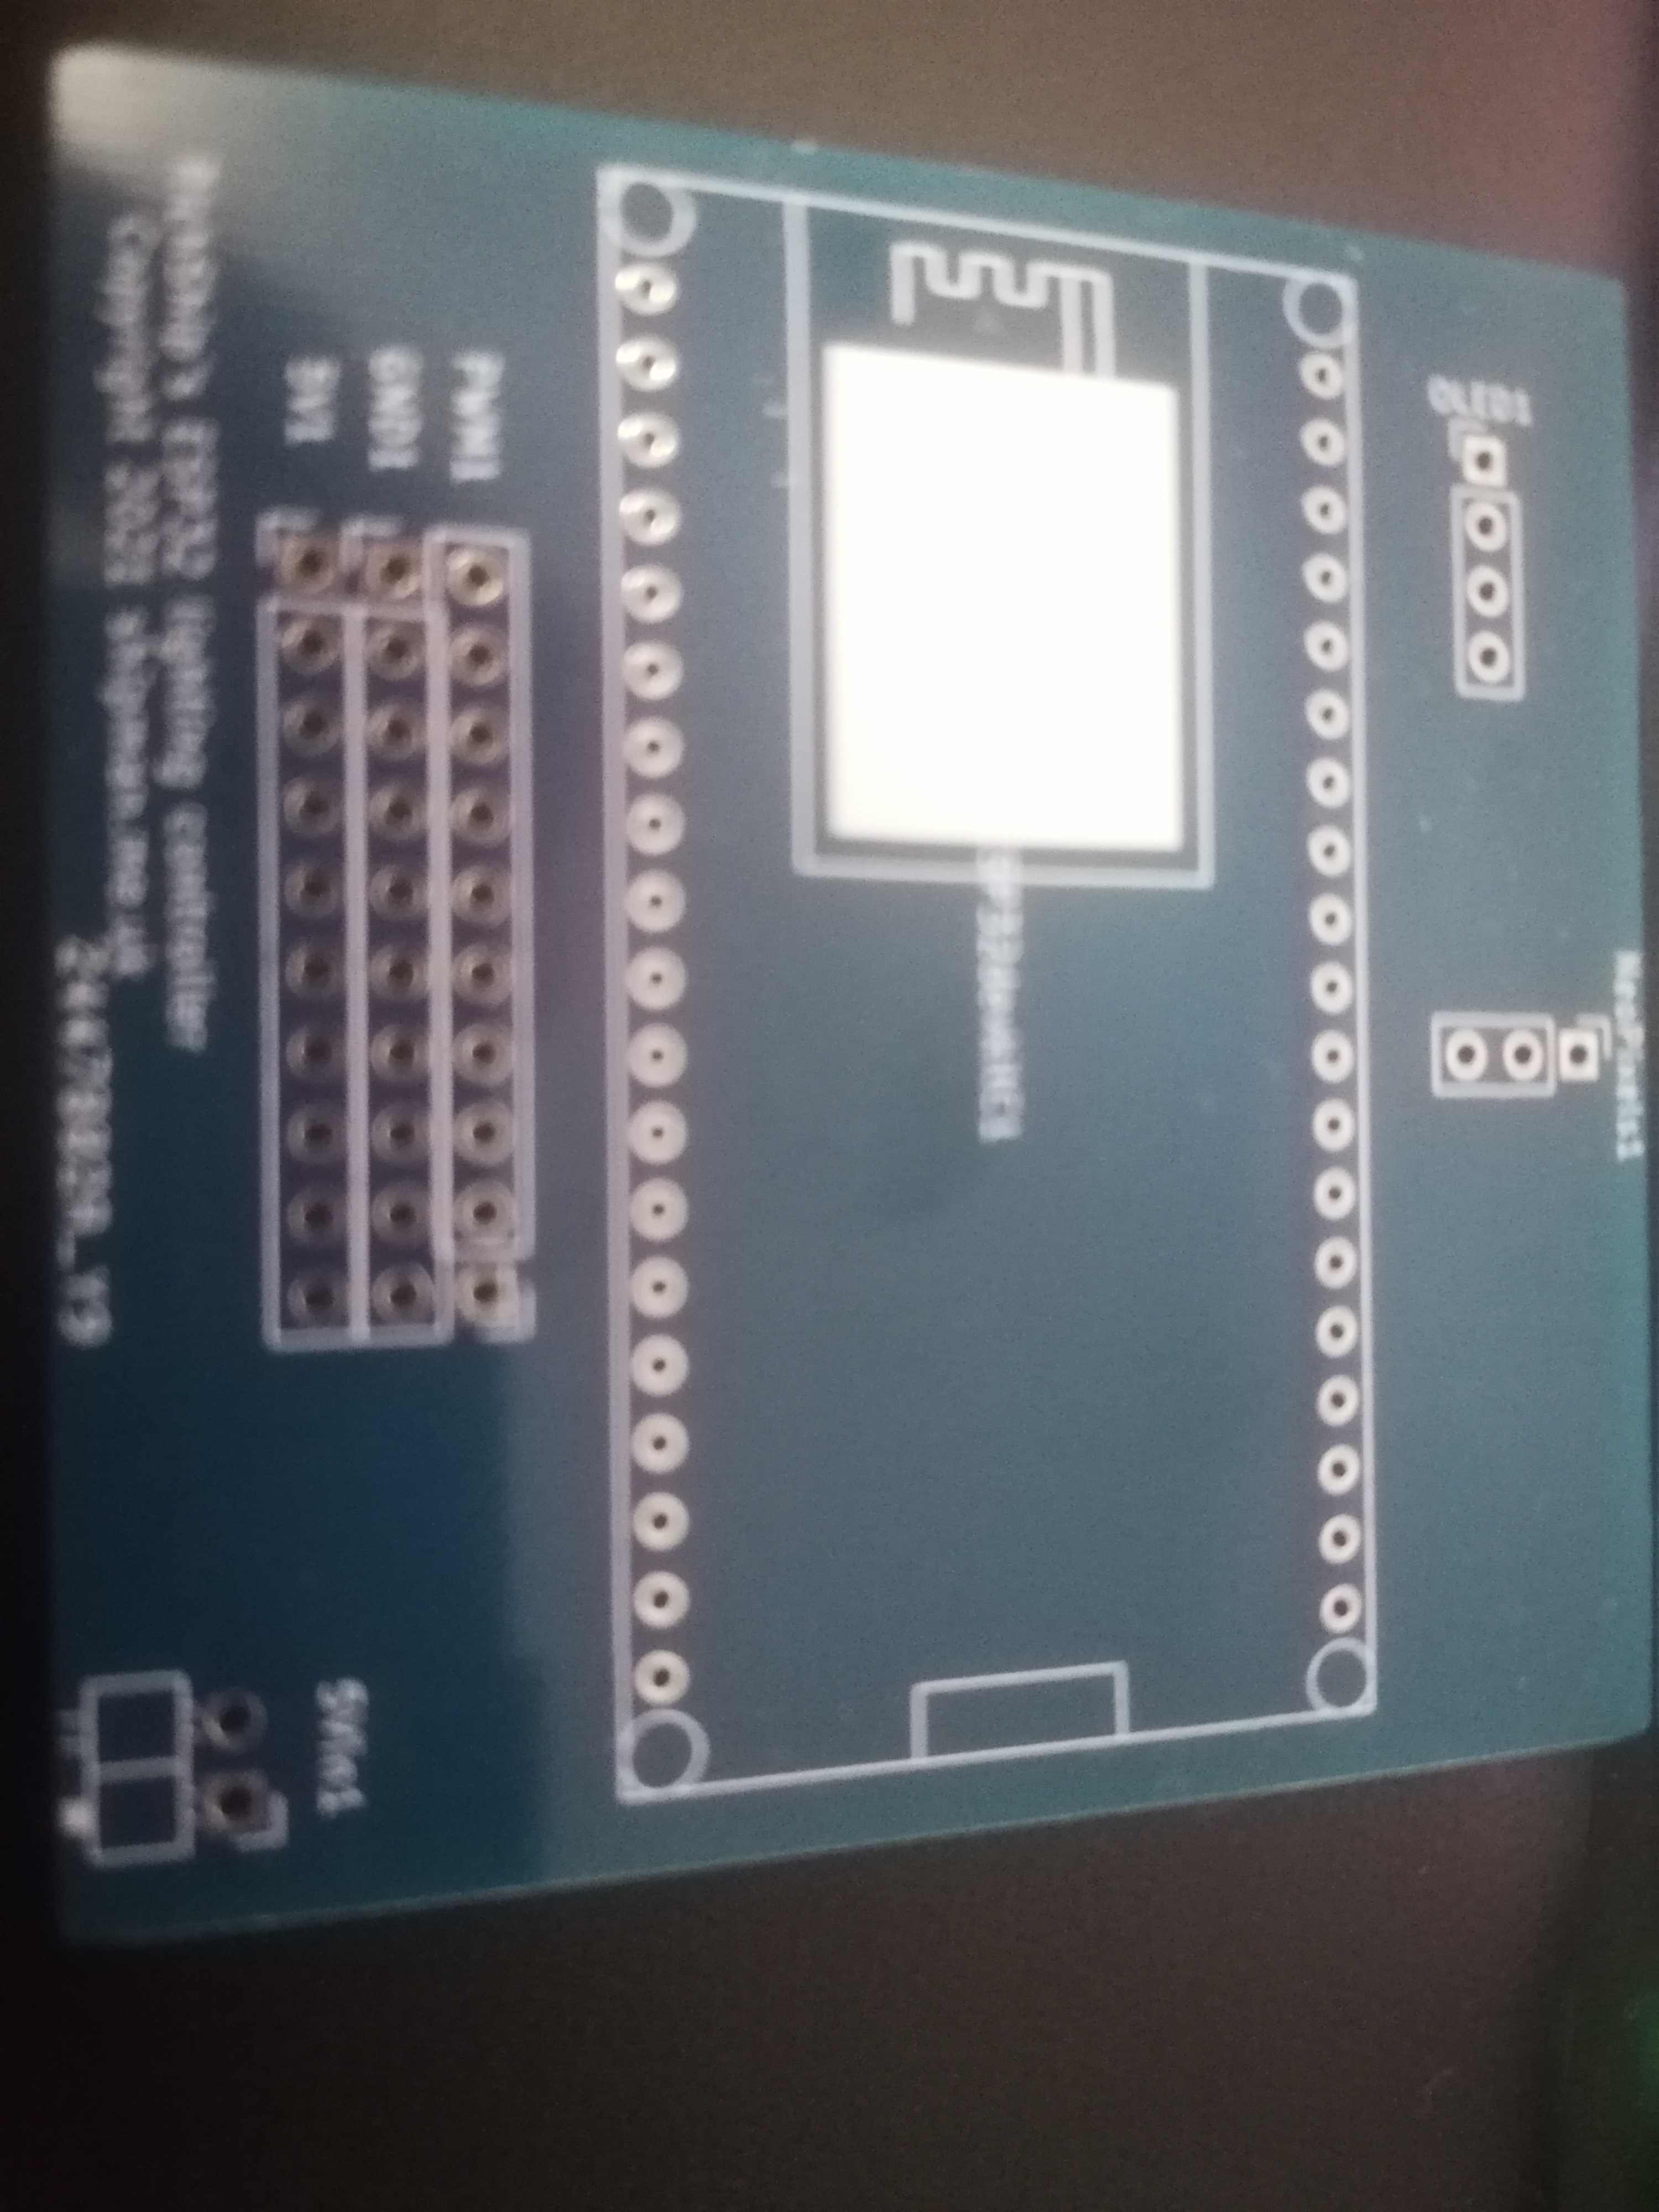
\includegraphics[width=6cm, height=6cm]{CircuitBoard}
\end{figure}


\section {Website Creation (Sprint Four)}
Before the beginning of the project, the complexity of HTML and CSS was underestimated on my part. Initially, the plan was to use file management within the ESP32 to have a document for the code, a document for the CSS style sheet and a document for the HTML sheet. After struggling with the concept of communication between the HTML webpage and the code for a couple of days which delayed the production of other parts of the code, it was decided that the HTML would be coded in the C++ file which is not as efficient as HTML but does work effectively enough for this design. 

\subsection{Website Simplification}
Due to bad planning and not keeping to the Scrum methodology as the project went on, there was not enough time left on the project to fully complete the web side of the project. Therefore, there was some sacrifices that had to be made to the functionality and the design of the website to allow for a semblance of a completed website.

\subsubsection{Functionality changes}
When the fourth sprint started, it was realised pretty quickly that the time scale left for the project did not allow for the time needed to implement all of the must have features identified in the MoSCoW analysis. So in order for a functioning website to be made, the functionality that was excluded from the website was the creation of the profiles. This was an undesirable but necessary step this far into the project with the time scale left in the project. Now, to create a profile the user must code it in the setup of the code. 

\subsubsection{Design chagnes}
When it came to the implementation of being able to change the triggers of the LED profiles on the website, there was some difficulties getting the dropdown boxes communicating what was selected to the main code. It was realised that you are unable to add ‘<a href>’ statements to the dropdown box implemented and to do it this way, a lot of CSS styling and HTML defining of drop-down boxes had to be made. As the time left before the project deadline was short and functionality had already been cut from the website, it was decided that the functionality of the website was more important than the look of the website. So instead of using drop-down boxes, simple links were implemented instead as a bad looking but functional website is better than a good looking one that does nothing.  

\begin{figure}[h]
\centering
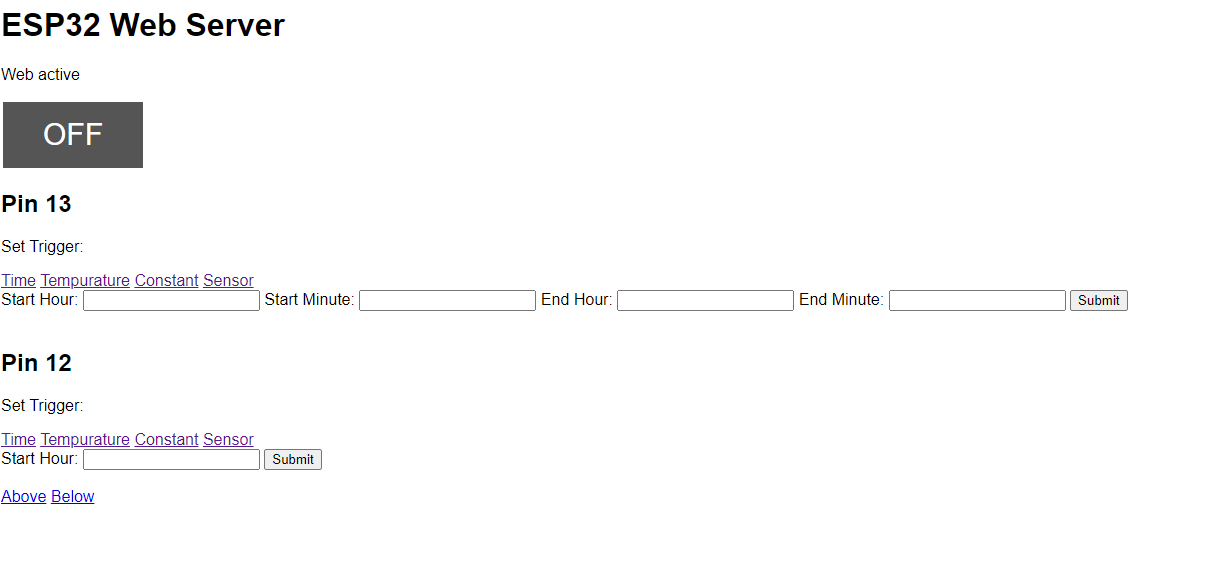
\includegraphics[width=17cm, height=13cm]{WebExample}
\end{figure}
